\chapter{Approach}
\label{chp:apr}
This chapter explains the general structure and functionality of a system that measures the received signal strength (RSS) of every link in a multi-hop Wireless Sensor Network (WSN). First, the chapter gives an overview of the general structure of the system. Then each individual task of the system is explained in detail.

\section{General Structure}
\label{chp:apr_general}

To measure the received signal strength (RSS) of each link, all the nodes need to send messages. Since two nodes sending a message at the same time distorts the RSS measurements, we need to make sure that only one node sends a message at a given point in time. One approach to achieve this is the multi-spin method that defines a time slot for each node according to its ID, so the nodes know when to send their message. However this method does not work inside a multi-hop WSN since it relies on the fact that every node can hear all the other nodes. This makes a different approach necessary that schedules the nodes and collects the data from the WSN. A similar approach would come to mind that also uses defined time slots but includes the collection and synchronization needed for it to work inside a multi-hop WSN. However, a problem with such a time slot based system is that when using a platform like TinyOS, where no full control over the execution of events and tasks is given, time slots cannot be defined accurately. This means, the time slots need to include an error that takes into account that a receive event does not necessarily gets triggered when the message was received.
 
To eliminate the delay time slots bring along, a different approach is suggested in this thesis which is based on predefined predecessors for each node. Based on this, each node is able to send a message directly after receiving a message from its predecessor still ensuring that only one node sends at a given point in time. Moreover each measurement $cycle$ is divided into a sampling and a collection phase making it possible for the approach to be used inside a multi-hop WSN.

The approach requires a WSN in which one node functions as the sink. The sink is connected to a base station with high processing power and a lot of storage. The structure of the WSN is represented in Figure \ref{fig:architecture}. Since the requirement for the approach is that it works inside a multi-hop WSN, it is a challenge to collect data from the network and to create a fitting schedule that defines predecessors for all the nodes inside the network. To be able to do so, a first calibration phase is needed to create paths from every node to the sink and collect information about the connections between nodes. Then the information about the connections needs to be collected at the sink and sent to the base station in a collection phase. When the base station has received all the information, it can create the schedule. After that the base station has to send the schedule to the sink that starts spreading it inside the network. 

Is the schedule spread and all the nodes know when to send their messages, the sampling of the RSS can start. Therefore messages are sent according to the predecessors defined in the schedule. All the nodes receiving the messages are now able to measure the received signal strength to the sending node and store this information. When the schedule is completed, another collection of the data is needed to gather the measured RSS at the base station for further processing. When the collection is done, the system can start sampling again and then again collect the data until the system is stopped. This process is shown in Figure \ref{fig:processes}.    

\begin{figure}[]
	\centering
	\begin{subfigure}[t]{0.4\textwidth}
		\centering
    		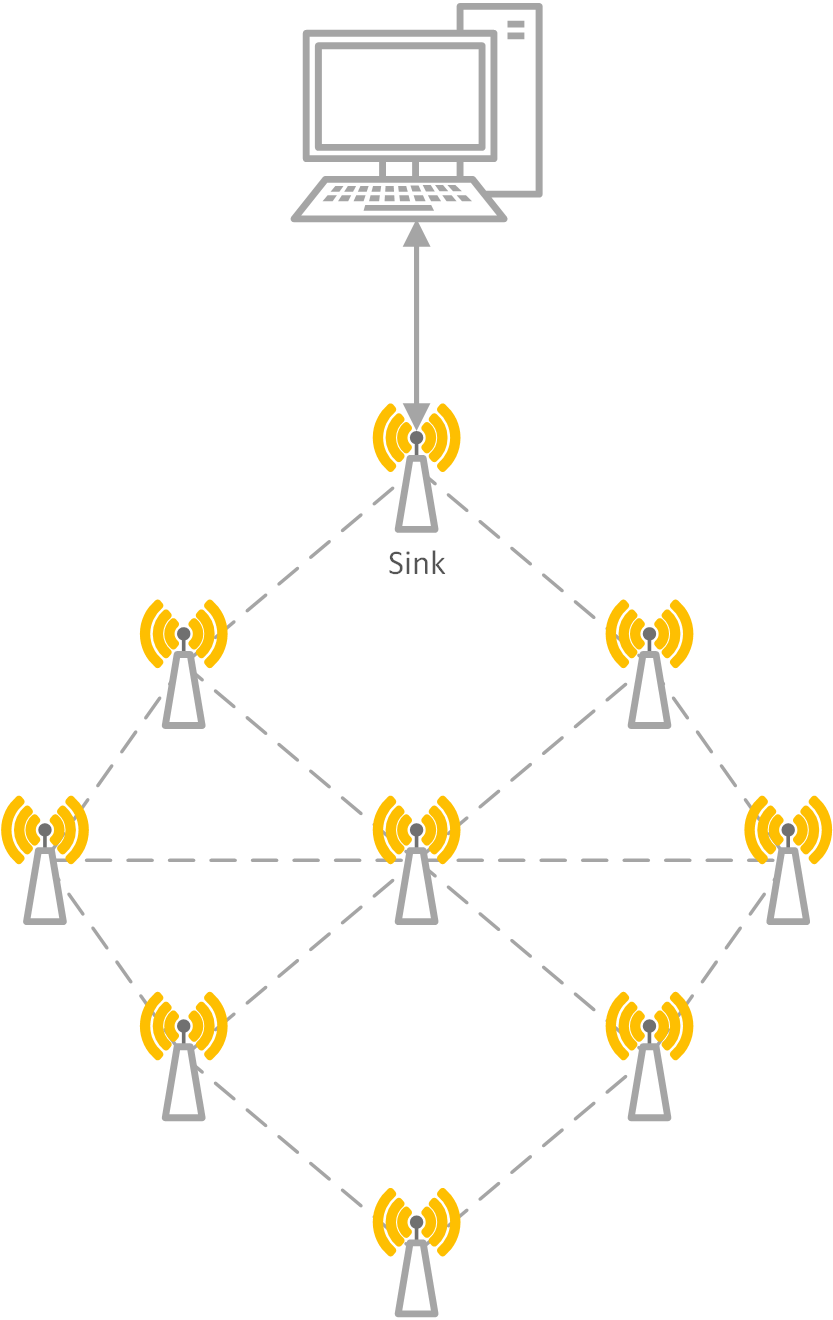
\includegraphics[scale=0.6]{content/images/Architecture}
   	 	\caption{The physical architecture of the system.}
    	\label{fig:architecture}
    \end{subfigure}
    \quad
    \quad
    \quad
    \begin{subfigure}[t]{0.4\textwidth}
		\centering         
        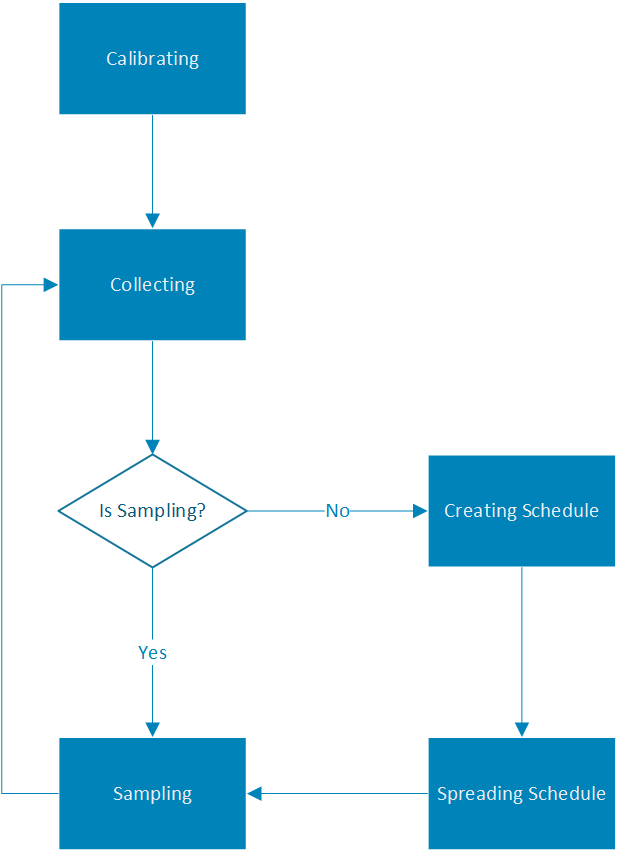
\includegraphics[scale=0.7]{content/images/GeneralAproachM}
        \caption{The general processes and the order in which they are executed.}
        \label{fig:processes}
    \end{subfigure}
    \caption{}
\end{figure}
  
\section{Calibration}
\label{chp:apr_calibration}
The calibration has two tasks. It needs to figure out for each node individually which nodes a node has in its range and it needs to create paths to the sink. These paths are used later to send data to the sink and to spread information inside the network. To achieve these tasks, each node broadcasts multiple messages without any specific pattern, meaning they do not need to take into account that messages can collide.

Each node needs to be able to keep track of the nodes in range. Therefore each node needs to have its own neighbour table. When a node receives a message, it can put the node it received the message from inside that neighbour table. All the neighbour tables will later be the basis to create the schedule.

To later collect data from each individual node at the sink, each node needs to know to which node it needs to send its data to so it will reach the sink. This node is the parent of the node. Moreover to spread data inside the network, each node also needs to know which nodes send to itself in direction of the sink. These nodes are the children of a node. When each node has found its parent and its children, all the paths together form a tree structure with the sink as the root.

To find the parents for the nodes, each node needs to save one extra information and also include this information inside the messages it sends. This information is the quality of the current path a node has to the sink. At the beginning all the nodes except the sink initialize their path quality with the worst possible value. The sink initializes its path quality with the best possible value. Now when a node receives a message, it adds to the received path quality of the sending node the quality of the link between itself and the sending node. The result is the path quality to the sink for the node, when it chooses the sending node as its parent. The quality of a link is represented by the received signal strength. When the new path quality is calculated, the node compares the calculated value with its current path quality. If the calculated value is better, the node sets its parent to the sending node and saves the new path quality. 

Now, to not only know the direction to the sink but also the dissemination from the sink to the whole network, the nodes need to find their children. Therefore each node simply includes their own parent inside the message it sends. A receiving node checks if it is the parent of the sending node. If that is the case, the receiving node can save the sending node as a child.       

\section{Collection}
\label{chp:apr_collection}

\begin{figure}[htbp]
	\centering
	\begin{subfigure}[t]{0.4\textwidth}
		\centering
    		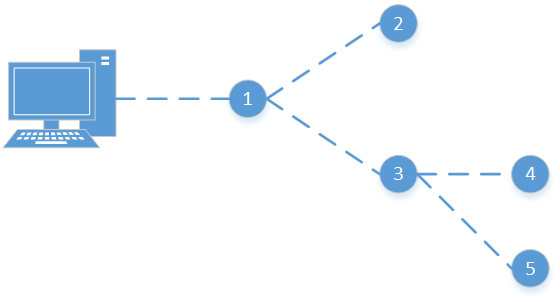
\includegraphics[scale=0.6]{content/images/Collection/Part0}
   	 	\caption{At the beginning all the nodes are unmarked and still have data to send.}
    	\label{fig:coll0}
    \end{subfigure}
    \quad
    \quad	
	\begin{subfigure}[t]{0.4\textwidth}
		\centering
    		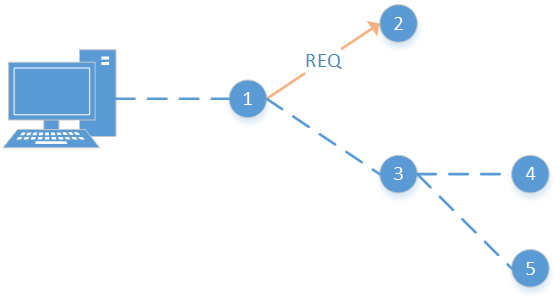
\includegraphics[scale=0.6]{content/images/Collection/Part1}
   	 	\caption{Node 1 sends the first request to node 2.}
    	\label{fig:coll1}
    \end{subfigure}
    \quad
    \quad
    \begin{subfigure}[t]{0.4\textwidth}
		\centering         
        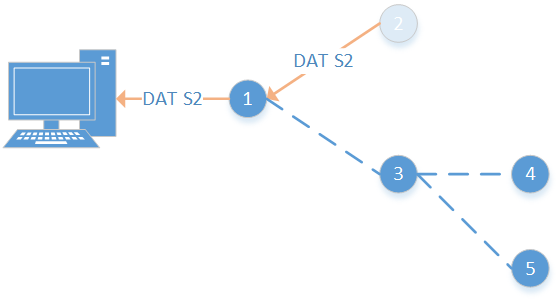
\includegraphics[scale=0.6]{content/images/Collection/Part2}
        \caption{Node 2 does not have any children, so it sends its data and gets marked.}
        \label{fig:coll2}
    \end{subfigure}
    \quad
    \quad
    \begin{subfigure}[t]{0.4\textwidth}
		\centering         
        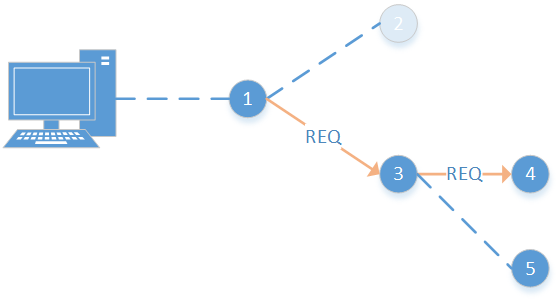
\includegraphics[scale=0.6]{content/images/Collection/Part3}
        \caption{Now node 2 is marked, so node 1 sends a request to node 3, which forwards it to node 4.}
        \label{fig:coll3}
    \end{subfigure}
    \quad
    \quad
    \begin{subfigure}[t]{0.4\textwidth}
		\centering         
        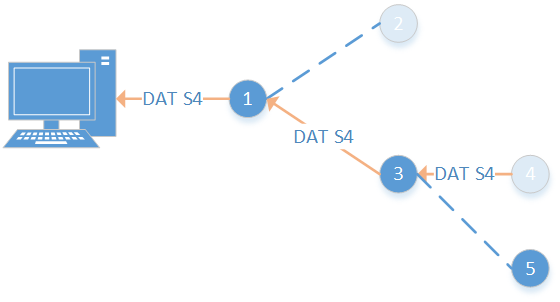
\includegraphics[scale=0.6]{content/images/Collection/Part4}
        \caption{Node 4 does not have any children, so it sends its data and gets marked.}
        \label{fig:coll4}
    \end{subfigure}
    \quad
    \quad
    \begin{subfigure}[t]{0.4\textwidth}
		\centering         
        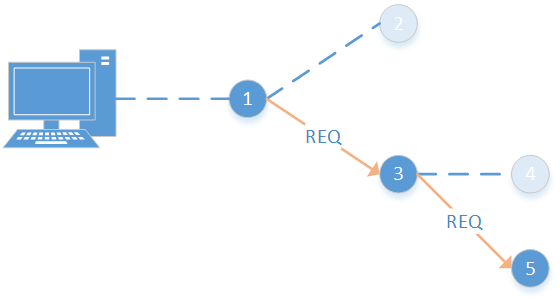
\includegraphics[scale=0.6]{content/images/Collection/Part5}
        \caption{Node 3 is still not marked, so node 1 sends a request to it. Node 4 is marked so node 3 forwards the request to node 5.}
        \label{fig:coll5}
    \end{subfigure}
    \quad
    \quad
    \begin{subfigure}[t]{0.4\textwidth}
		\centering         
        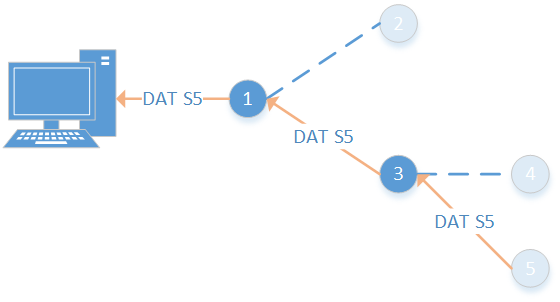
\includegraphics[scale=0.6]{content/images/Collection/Part6}
        \caption{Node 5 does not have any children, so it sends its data and gets marked.}
        \label{fig:coll6}
    \end{subfigure}
    \quad
    \quad
    \begin{subfigure}[t]{0.4\textwidth}
		\centering         
        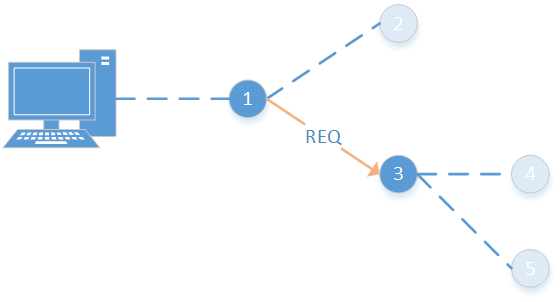
\includegraphics[scale=0.6]{content/images/Collection/Part7}
        \caption{Node 3 is still not marked, so node 1 sends a request to it.}
        \label{fig:coll7}
    \end{subfigure}
    \quad
    \quad
    \begin{subfigure}[t]{0.4\textwidth}
		\centering         
        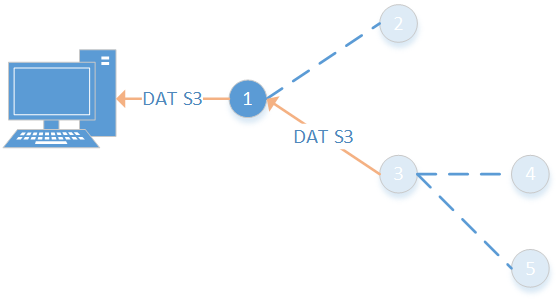
\includegraphics[scale=0.6]{content/images/Collection/Part8}
        \caption{All the children of node 3 are marked, so it starts sending its data and gets marked itself.}
        \label{fig:coll8}
    \end{subfigure}
    \quad
    \quad
    \begin{subfigure}[t]{0.4\textwidth}
		\centering         
        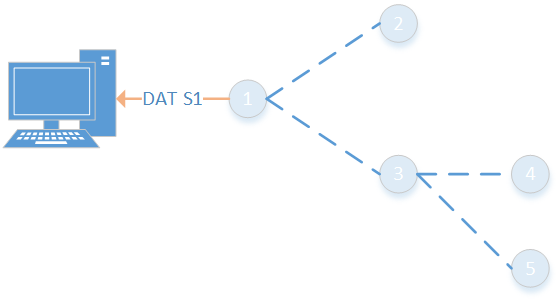
\includegraphics[scale=0.6]{content/images/Collection/Part9}
        \caption{Now all the children of node 1 are marked and it can send its own data to the base station and gets marked.}
        \label{fig:coll9}
    \end{subfigure}
    \caption{This is an example for the collection. REQ means request and DAT Sx stands for data from source x.}
    \label{fig:coll}
\end{figure}

To collect the data from the network, we make use of the created paths and their tree structure. The process is shown in Figure \ref{fig:coll}. The Figure shows a Wireless Sensor Network represented by the nodes and the paths to the sink created in the calibration phase. Note that the nodes could also have other connections between each other. 

To start the collection, the sink sends a request to one of its children. The child receiving that request checks if it has any children itself and if that is the case, it forwards the request to one of them. When the request reaches a node without any children, the node sends its data to its parent which forwards the data to its parent, until the data reaches the sink, which forwards it to the base station. Every node that receives a data message, locally marks the source node of that data as done. When the sink has sent the received data to the base station, it sends a new request to one of its children that has not been marked as done. That child again forwards that request to a child that has not been marked as done. If the request reaches a node that has no children or every child has been marked as done, it sends its own data. This process will be repeated until the sink does not have any more children left that are not marked as done. Then the sink can send its own data to the base station and finish the collection. All nodes now need to unmark all the other nodes, so another collection is possible.

Since a node only sends its data when it receives a request created by the sink, the sink is able to control when the collection starts and when it ends. This makes it possible to split the collection and the sampling, preventing distortion of the signal strength measurements. This would not be possible with a protocol like the Collection Tree Protocol that does not provide any control over the collection procedure. 

\section{Creating the Schedule}
\label{chp:apr_creatingSchedule}
A fitting schedule is a path through the graph structure of the WSN that visits every node at least once and starts and ends at the same node. The schedule needs to form a circle because the sink needs to collect the data after each round. This means the sink needs to know when every node has sent its message which is the case when it is the last node in the schedule. Since the sink also knows when the collection is done, it makes sense that it starts the next round and therefore is also the first node of the schedule. 

The optimal schedule would be a Hamilton-Circle, which is a circle inside a graph that visits each node exactly once. To figure out if a Hamilton-Circle exists, it is only possible to bruteforce all the possible combinations. This is highly inefficient and possibly we do not even get a result at the end. Therefore this thesis suggests a simple method that makes sure every node gets visited at least once and the path starts and ends at the same node. This method however is not able to create an optimal schedule.

\subsection{Rooted Circles}
\begin{figure}[htbp]
	\centering
	\begin{subfigure}[t]{0.4\textwidth}
		\centering
    		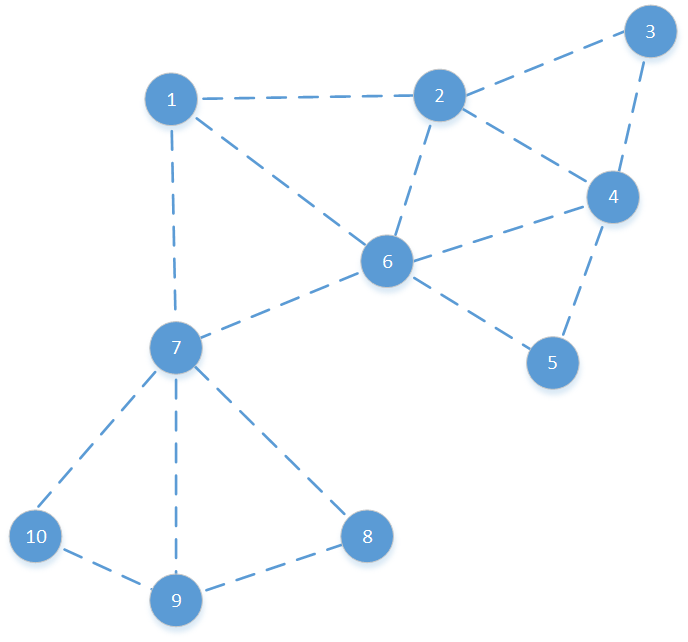
\includegraphics[scale=0.6]{content/images/Schedule/Network}
   	 	\caption{The example network with all its connections between nodes.}
    	\label{fig:network}
    \end{subfigure}
    \quad
    \quad
    \begin{subfigure}[t]{0.4\textwidth}
		\centering         
        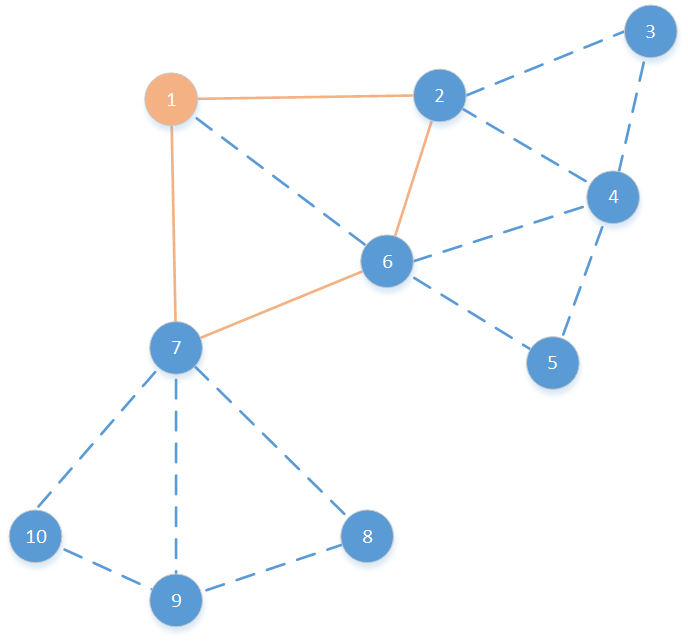
\includegraphics[scale=0.6]{content/images/Schedule/RootedCircle}
        \caption{Example for a rooted circle with node 1 as the root.}
        \label{fig:rootedCircle}
    \end{subfigure}
    \label{fig:networkRootedCircle}
    \caption{A rooted circle inside an example network.}
\end{figure}

The suggested method is based on smaller circles inside the graph. These circles have a root node that is the start and the end point of the circle. All the nodes inside this circle are in range of the root of the circle. These circles will be called rooted circles. In Figure \ref{fig:rootedCircle}, such a rooted circle is represented inside the network depicted in Figure \ref{fig:network}. To create a rooted circle, one node needs to be chosen as the root. Then the base station takes one node from the root's neighbour table and chooses it as the second node in the circle.  Then the base station looks into the second node's neighbour table and chooses a node that has the root node inside its neighbour table as the next node in the circle. The base station then does the same for the chosen node and this process is repeated until one node does not have a neighbour that has also the root as a neighbour. Then the circle is closed and the path goes back to the root. When we look at the example in Figure \ref{fig:rootedCircle}, this means node 1 was chosen as the root. Then node 2 was picked as the second node in the circle. Node 2 has multiple neighbours but only one of them, node 6, has the root node 1 as a neighbour. This means node 6 is chosen as the next node in the circle. Node 6 now has node 2 and node 7 as neighbours that also have the root as a neighbour, however node 2 is already inside the circle so node 7 is chosen as the next node. Node 7 now has no more neighbours that have the root as a neighbour and the circle is closed.

\subsection{Creating a Full Schedule}
\begin{figure}[htbp]
	\centering         
    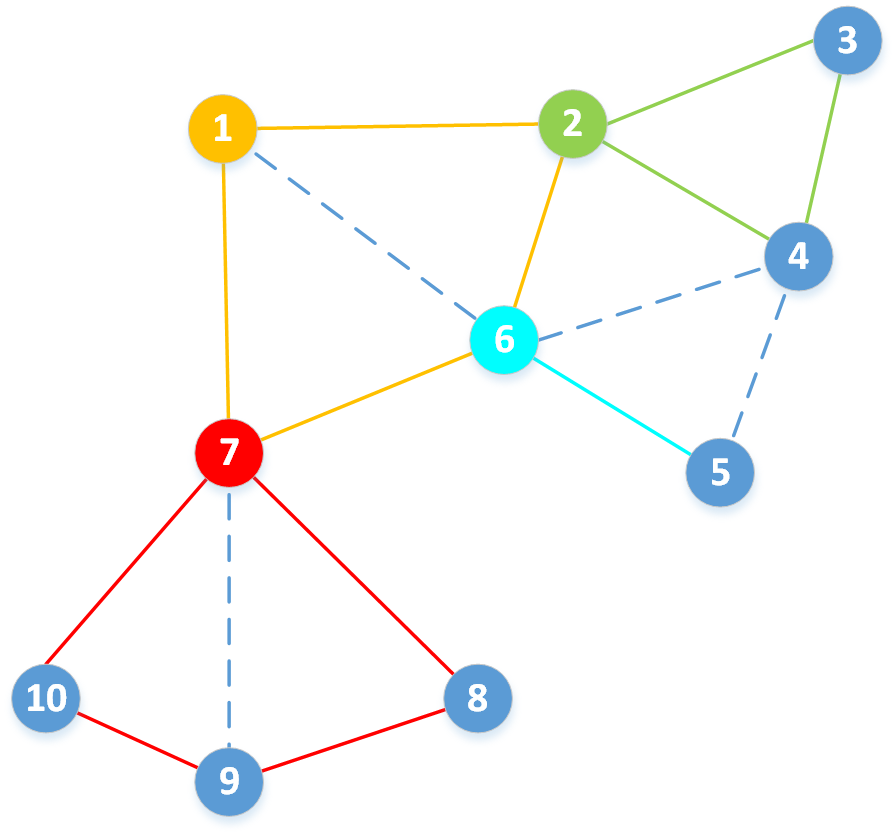
\includegraphics[scale=0.6]{content/images/Schedule/FullSchedule}
    \caption{Full schedule for the example network of Figure \ref{fig:network}. The order in which the nodes send their messages would be: 1 2 3 4 2 6 5 6 7 8 9 10 7 1.}
    \label{fig:schedule}
\end{figure} 
To create a full schedule, the whole graph needs to be filled with rooted circles. Therefore the base station chooses the sink as the first root and creates a rooted circle around it. When the circle is done, the base station goes through all the nodes of the circle and, if possible, creates rooted circles around them as well. Then we do the same for all the new circles until every node was suggested as a root once. When creating new circles, it is not possible to choose a node already inside another circle to be part of the new circle. In Figure \ref{fig:schedule} the network from Figure \ref{fig:network} is fully covered by rooted circles. The first circle created was the one that has node 1 as a root. Then all the nodes inside that circle were chosen as new roots to create new rooted circles. The first thing one could notice is that the circle with the root 6 only has one other node and does not really form a circle. This happens if the circle is closed directly after the second node following the root is chosen because there are no more neighbours left that also have the root as a neighbour. When running the schedule, this means a message would be sent from node 6 to node 5 and then from node 5 back to node 6. Also note that in theory there is a bigger rooted circle possible with the root 6 when node 4 would be included, but the rooted circle with the root 2 was created first and included node 4, blocking it for rooted circles created at a later point in time. Listing 3.1 provides the pseudocode of an algorithm to cover a whole graph with rooted circles.

\lstset{caption={Pseudocode that covers a graph with rooted circles.},label={lis:rooted}}
\begin{lstlisting}
RootedCircle createRootedCircle(Node root) {
	Node node = getNextForCircle(root, root)	

	If(node != null) {
		RootedCircle rootedCircle = new rootedCircle(root)
		rootedCircle.addNode(node)
		node.setPartOfCircle(true)

		while((node = getNextForCircle(root, node, rootedCircle)) != null) {
			rootedCircle.add(node)
			node.setPartOfCircle(true)
		}

		return rootedCircle
	} else {
		return null
	}
}

Node getNextForCircle(Node root, Node neighbour) {
	for each (Node node in root.getNeighbourList)	
		if(node.isNeighbourOf(neighbour) and not node.isPartOfACircle())
			return node
	return null
}

List<RootedCircle> coverGraphWithRootedCircles(Node firstRoot) {
	List<RootedCircle> circleList = new List<RootedCircle()>
	
	circleList.add(createRootedCircle(firstRoot))

	for each (RootedCircle circle in circleList) {
		for each (Node node in circle) {
			RootedCircle newCircle = createRootedCircle(node)
			if(newCircle != null)
				circleList.add(newCircle);
		}
	}
}
\end{lstlisting}

\section{Spreading the Schedule}
\label{chp:apr_spreadingSchedule}
To spread the schedule, we are again making use of the tree structure of the created path. When the sink received the schedule from the base station, it forwards it to its first child. The child forwards it to one of his children and so on. When a node that received the schedule has no more children, it sends the schedule back to its parent. The parent receiving the schedule now forwards the schedule to its next child. If a parent received the schedule back from all its children, it forwards it to its own parent. In Figure \ref{fig:spreading} an example for this process is given. The Figure shows a Wireless Sensor Network represented by the nodes and the paths to the sink created in the calibration phase. Note that the nodes could also have other connections between each other. 

When looking at the example, one can see that already in Figure \ref{fig:spreading7} the schedule is received by all the nodes but still there are messages sent that could seem useless at this point. However at this point in time it is not known if the sink has any more children that did not receive the schedule yet. Therefore the schedule needs to travel all the way back to the sink. Only at the moment the schedule reaches the sink and the sink does not have any more children left that need to receive the schedule, it is sure that the schedule is fully spread.

\begin{figure}[htbp]
	\centering
	\begin{subfigure}[t]{0.4\textwidth}
		\centering
    		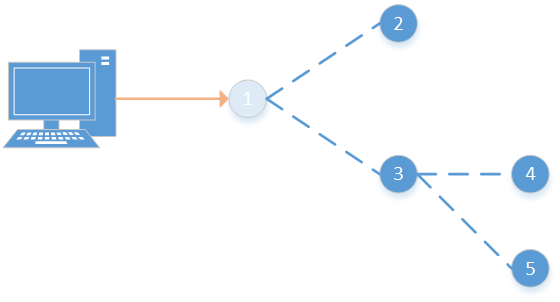
\includegraphics[scale=0.6]{content/images/ScheduleSpreading/Part1}
   	 	\caption{The base station sends the schedule to node 1.}
    	\label{fig:spreading1}
    \end{subfigure}
    \quad
    \quad
    \begin{subfigure}[t]{0.4\textwidth}
		\centering         
        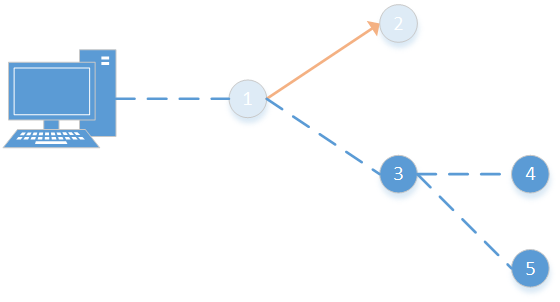
\includegraphics[scale=0.6]{content/images/ScheduleSpreading/Part2}
        \caption{Node 1 forwards the schedule to node 2.}
        \label{fig:spreading2}
    \end{subfigure}
    \quad
    \quad
    \begin{subfigure}[t]{0.4\textwidth}
		\centering         
        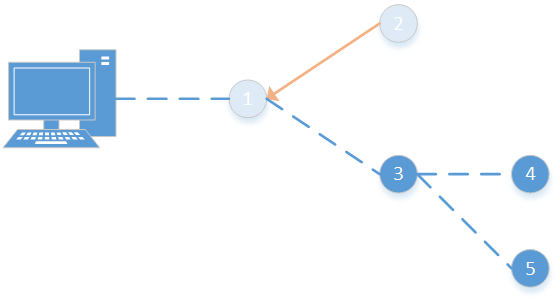
\includegraphics[scale=0.6]{content/images/ScheduleSpreading/Part3}
        \caption{Node 2 does not have any children and sends the schedule to its parent node 1.}
        \label{fig:spreading3}
    \end{subfigure}
    \quad
    \quad
    \begin{subfigure}[t]{0.4\textwidth}
		\centering         
        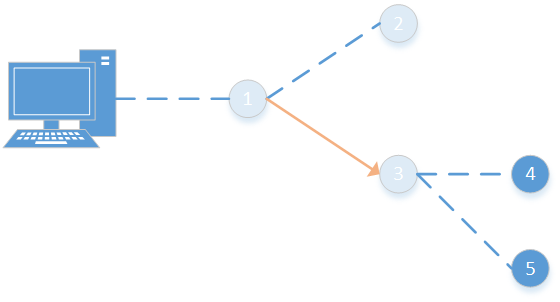
\includegraphics[scale=0.6]{content/images/ScheduleSpreading/Part4}
        \caption{Node 2 is now marked so node 1 forwards the schedule to node 3.}
        \label{fig:spreading4}
    \end{subfigure}
    \quad
    \quad
    \begin{subfigure}[t]{0.4\textwidth}
		\centering         
        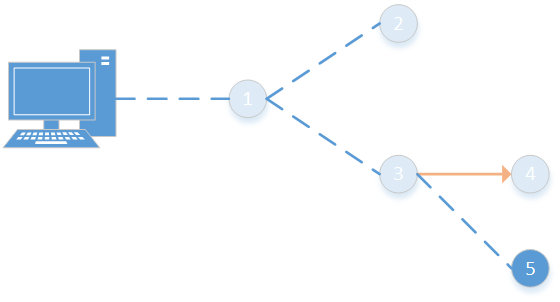
\includegraphics[scale=0.6]{content/images/ScheduleSpreading/Part5}
        \caption{Node 3 forwards the schedule to node 4.}
        \label{fig:spreading5}
    \end{subfigure}
    \quad
    \quad
    \begin{subfigure}[t]{0.4\textwidth}
		\centering         
        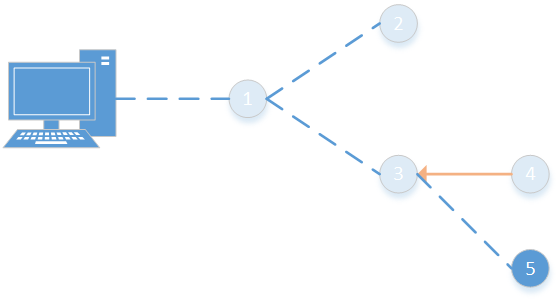
\includegraphics[scale=0.6]{content/images/ScheduleSpreading/Part6}
        \caption{Node 4 does not have any children and sends the schedule to its parent node 3.}
        \label{fig:spreading6}
    \end{subfigure}
    \quad
    \quad
    \begin{subfigure}[t]{0.4\textwidth}
		\centering         
        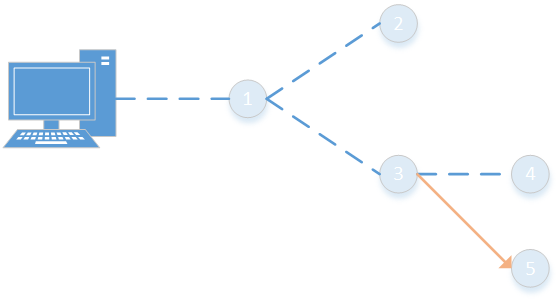
\includegraphics[scale=0.6]{content/images/ScheduleSpreading/Part7}
        \caption{Node 3 has still node 5 as an unmarked child and forwards the schedule to it.}
        \label{fig:spreading7}
    \end{subfigure}
    \quad
    \quad
    \begin{subfigure}[t]{0.4\textwidth}
		\centering         
        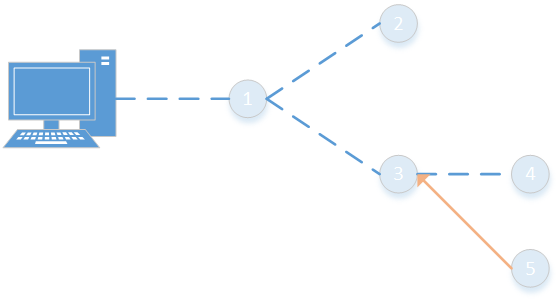
\includegraphics[scale=0.6]{content/images/ScheduleSpreading/Part8}
        \caption{Node 5 does not have any children and sends the schedule to its parent node 3.}
        \label{fig:spreading8}
    \end{subfigure}
    \quad
    \quad
    \begin{subfigure}[t]{0.4\textwidth}
		\centering
    		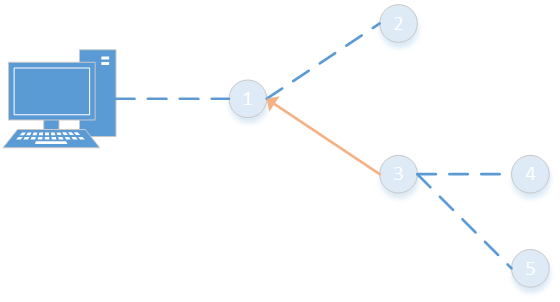
\includegraphics[scale=0.6]{content/images/ScheduleSpreading/Part9}
   	 	\caption{Node 3 has no more unmarked children and sends the schedule to its parent node 1.}
    	\label{fig:spreading9}
    \end{subfigure}
    \quad
    \quad	
    \begin{subfigure}[t]{0.4\textwidth}
		\centering         
        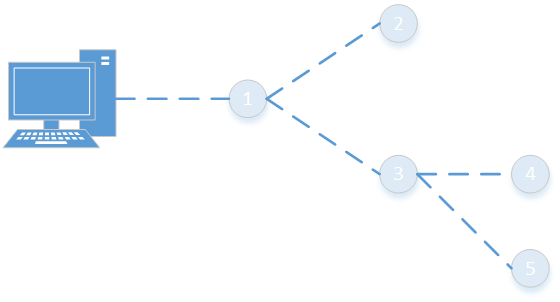
\includegraphics[scale=0.6]{content/images/ScheduleSpreading/Part10}
        \caption{Since node 1 does not have any more unmarked children, the schedule is now fully spread inside the network.}
        \label{fig:spreading10}
    \end{subfigure}
    \caption{This is an example for a path a schedule message takes to be spread inside the network.}
     \label{fig:spreading}
\end{figure}

\subsection{Sampling}
\label{chp:apr_sampling}
When all nodes received the schedule, it is possible to sample the received signal strength by sending messages according to it. Therefore the sink starts broadcasting a message. When its successor receives the message, it can broadcast its own message and so on until the last message was sent and the sampled data can be collected. However we need to take into account that we do not have a perfect schedule where every node only appears once, meaning a node could have multiple predecessors and successors. Therefore we need to include the successor of the sending node inside the message so a receiving node can see if he is the correct successor at that moment and evaluate the correct successor for itself. 
\subsection{Message Drops}
\label{chp:apr_samplingDrops}
\begin{figure} [htbp]
	\centering         
    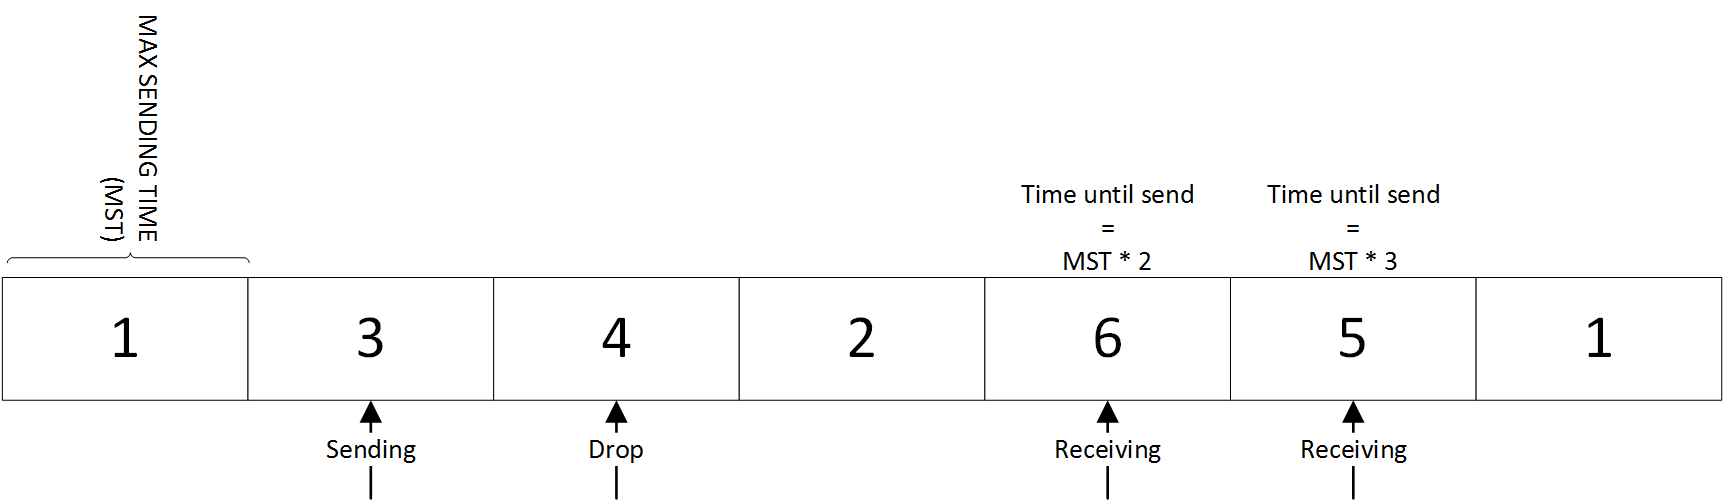
\includegraphics[scale=0.6]{content/images/MessageDrop}
    \caption{Representation of a schedule. Node 3 sends a message. Node 4 drops the message but node 6 and 5 receive it so that they can calculate the time when they should send.}
    \label{fig:msgDrop}
\end{figure}
A problem of the proposed method are message drops. If a successor does not receive the message of its predecessor, the whole system would stop. Here, a technique similar to a time slot based system like Multi-Spin uses comes in handy. For this method every node needs to know the whole schedule and not only its own predecessors and successors. Then whenever a node receives a message, it can look up how many nodes need to send between the node that just sent and itself. Then the amount of sending nodes is multiplied by the maximal time a node needs to send a message. The result is the time after the node can send its own message, without receiving a message from its predecessor. This procedure is shown in an example in Figure \ref{fig:msgDrop}. The Figure shows a simple schedule. Node 3 sends a message but the successor node 4 does not receive it. However node 6 and 5 receive the message and can therefore calculate the times they need to wait until they can send their messages. However, since node 4 has not received a message yet, it is not able to send a message and the same applies to node 2. 

Again we need to take into account that a node can appear multiple times in the schedule. Therefore after a node has sent a message, it needs to calculate the maximal time until it can send its next message.